\chapter{Instrumental Inequality and beyond}
\label{ch-inst-ineq}

This chapter is based on
Refs. \cite{evans-inst-ineq} and 
\cite{pearl-inst-ineq}.

Instrumental Variables (IVs) 
are discussed in Chapter \ref{ch-instrumental}.
This chapter will discuss
the original Instrumental
inequality (I-inequality)
discovered by Pearl, 
and other related inequalities.
The I-inequality arises
in bnets that use an IV.
The I-inequality bounds
the effect that an IV
$\rvz$
can have on the outcome $\rvy$ of
a treatment $\rvd\rarrow\rvy$.
Since
there is a path
$\rvz\rarrow\rvd\rarrow\rvy$,
the treatment dose $\rvd$
acts as a mediator
between the IV $\rvz$ 
and the treatment outcome $\rvy$.
The I-inequality is reminiscent
of the data processing 
inequality
$H(\rvz:\rvy)\leq H(\rvd:\rvy)$
which is valid
for a simple Markov chain bnet 
$\rvz\rarrow\rvd\rarrow\rvy$.
The data processing
inequality
is saying that
the endpoint $\rvy$
receives 
more information from $\rvd$
than from
$\rvz$. This is reasonable,
since $\rvy$ is ``closer" to $\rvd$ than to
$\rvz$.



\section{I-inequality}

\begin{figure}[h!]
$$
\begin{array}{ccc}
\xymatrix{
&&\rvu\ar@{-->}[dl]\ar@{-->}[dr]
\\
\rvz\ar[r]
&\rvd\ar[rr]&&\rvy
}
&&
\xymatrix{
&&\rvu\ar@{-->}[dl]\ar@{-->}[dr]
\\
\rvz\ar[r]
&\rvd
&\rvtd=\td\ar[r]
&\rvy
}
\\
\\
G&&\tilde{G}=\kappa_{\rvd\rarrow\rvy}(\td)G
\end{array}
$$
\caption{In bnet $G$, 
an IV $\rvz$
acts on a treatment $\rvd\rarrow\rvy$.
Bnet $\tilde{G}$
is obtained
by applying
an imagine
operator
to arrow
$\rvd\rarrow\rvy$
of bnet $G$.} 
\label{fig-iv-ineq-im}
\end{figure}

\begin{claim}
The TPMs for the bnet $G$ in 
Fig.\ref{fig-iv-ineq-im}
satisfy

\beq
\max_d \sum_y \max_z
P(d,y|z)
\leq 1
\eeq
\end{claim}
\proof

Below,
any
probability
that alludes
to a value $\td$
refers to bnet $\tilde{G}$.
Otherwise,
if it doesn't allude to $\td$, then
it refers to $G$
(or to $\tilde{G}$,
since the TPMs of $\tilde{G}$
are defined
from those
of $G$
in a consistent manner.)


$G$ satisfies
\beq
P(d,y|z)=\sum_u P(u)
P(y|u, d)P(d|u,z)
\;,
\label{eq-p-d-y-bar-z}
\eeq
and $\tilde{G}$ satisfies

\beq
P(d,y|z, \td)=\sum_u P(u)
P(y|u,\td)P(d|u,z)
\;.
\label{eq-p-d-y-bar-z-tilde}
\eeq
Note that Eqs.(\ref{eq-p-d-y-bar-z})
and
(\ref{eq-p-d-y-bar-z-tilde}) imply that

\beq
P(d,y|z, d)=P(d,y|z)
\eeq
and that


\beq
\boxed{
P(\td, y|z, \td)\leq \sum_d P(d, y|z, \td)
=P(y|\td)
}
\;.
\label{eq-p-td-boxed}
\eeq
Thus,

\beqa
\max_\td \sum_y\max_z P(\td, y|z, \td)
&\leq &\max_\td \sum_y\max_z P(y|\td)
\\
&\leq&\max_\td \sum_yP(y|\td)
\\
&\leq&\max_\td 1
\\
&\leq&1
\eeqa
\qed


As pointed out in Ref.\cite{evans-inst-ineq}
from which
I learned the above
proof,
the above proof
is highly
generalizable.

Fig.\ref{fig-iv-ineq-proof}
gives a graphical
representation
of the boxed
Eq.(\ref{eq-p-td-boxed})
which is crucial
to the proof.

\begin{figure}[h!]
$$
\begin{array}{cccccc}
\sum_u
\xymatrix{
&&\rvu\ar@{-->}[dl]\ar@{-->}[dr]
\\
\rvz\ar[r]
&\rvd=\td
&\rvtd=\td\ar[r]
&\rvy
}&\leq&
\sum_d  \sum_u
\xymatrix{
&&\rvu\ar@{-->}[dl]\ar@{-->}[dr]
\\
\rvz\ar[r]
&\rvd
&\rvtd=\td\ar[r]
&\rvy
}
&=&
\xymatrix{
.
\\
\rvtd=\td\ar[r]
&\rvy
}
\end{array}
$$
\caption{Graphical
representation
of the boxed equation
Eq.(\ref{eq-p-td-boxed}). } 
\label{fig-iv-ineq-proof}
\end{figure}

And here is a 
meta-description
of the steps in the proof:
\begin{enumerate}
\item Use imagine operator to create a
non-negative matrix $M_{d, \td}$.
\item Use fact that row or column sum
of $M_{d, \td}$ is larger than diagonal
element in sum: 
$\sum_d M_{d, \td}\geq M_{\td,\td}$.
\end{enumerate}

\subsection{I-inequality for 
binary z,d,y}


It is enlightening
to write down the
I-inequality 
for the special case that
$\rvz, \rvd, \rvy$
are binary.

\begin{figure}[h!]
\centering
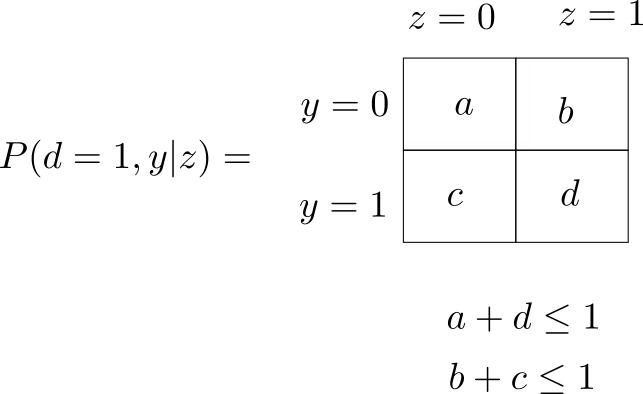
\includegraphics[width=3in]
{inst-ineq/binary-inst-ineq.png}
\caption{I-inequality for 
binary $\rvz, \rvd, \rvy$.
The same picture except with $d=0$
is also true.} 
\label{fig-iv-ineq-binary}
\end{figure}

In the binary case,
the I-inequality implies 4 different inequalities.
These are as follows.
One gets 
two inequalities 
by setting $d=1$ 
in the next 2 equations.

\begin{subequations}
\label{eq-i-ineq-bin}
\beq
\sum_{y=0}^1\sum_{z=0}^1 \indi(y=z) P(d,y|z)
\;,
\eeq

\beq
\sum_{y=0}^1\sum_{z=0}^1 
\indi(y\neq z) P(d,y|z)
\;.
\eeq
\end{subequations}
One gets an additional
2 inequalities by setting $d=0$
in Eqs.(\ref{eq-i-ineq-bin}).
These 4 inequalities
are illustrated in Fig.\ref{fig-iv-ineq-binary}.

What do they mean? That at fixed $\rvd$,
 the correlation
between $\rvz$ and $\rvy$ is limited.


\section{Bounds on 
Effect of IV on treatment
outcome y
}

\begin{figure}[h!]
$$
\begin{array}{ccccc}
\xymatrix{
&&\rvu\ar@{-->}[dl]\ar@{-->}[dr]
\\
\rvz\ar[r]\ar@/_1.5pc/[rrr]
&\rvd\ar[rr]&&\rvy
}
&&
\xymatrix{
&&\rvu\ar@{-->}[dr]
\\
\rvz\ar@/_1.5pc/[rrr]
&\rho\rvd=\td\ar[rr]&&\rvy
}
&&
\xymatrix{
&&\rvu\ar@{-->}[dl]\ar@{-->}[dr]
\\
\rvz\ar[r]\ar@/_1.5pc/[rrr]
&\rvd
&\rvtd=\td\ar[r]
&\rvy
}
\\
\\
\calg&&
\calg_{do}=\rho_{\rvd=\td}\calg
&&\calg_{im}=
\kappa_{\rvd\rarrow\rvy}(\td)\calg
\end{array}
$$
\caption{Bnet $\calg$
is obtained
from the bnet $G$
in Fig.\ref{fig-iv-ineq-im}
by adding to $G$ an arrow
from the IV $\rvz$
to the treatment
outcome $\rvy$.
Bnet $\calg_{do}$
is obtained by applying
a do operator
to node $\rvd$ of $\calg$.
Bnet $\calg_{im}$
is obtained by applying
an imagine operator
to arrow $\rvd\rarrow\rvy$ of $\calg$.
} 
\label{fig-iv-ineq-z-y-arc}
\end{figure}
In this section,
we will assume
that random variables
$\rvz, \rvd, \rvy$
are binary.
Just as with
the binary case
of the I-inequality,
we will
find an inequality
for each value
of $\rvd\in \bool$.

Below, we will
use the following 3
shorthand notations:

\beq
P_{y|z}(d)=
P(d,y|z)
\;,
\eeq

\beq
P_{|z}(d)=\sum_y P(d, y|z)
\;,
\eeq
and

\beq
\pi_{|z}(d) = 1-P_{|z}(d)
\;.
\eeq

For the bnet $\calg_{do}$
in Fig.\ref{fig-iv-ineq-z-y-arc},
define the IV effect at
fixed  $\rho\rvd=\td$ by
\beq
IVE(\td)=
P(y=1|z=1, \rho\rvd=\td)-
P(y=1|z=0, \rho\rvd=\td)
\;.
\eeq

\begin{claim}
The TPMs for the bnet $\calg_{do}$
in Fig.\ref{fig-iv-ineq-z-y-arc}
 satisfy

\beq
\pi_{|0}(d)\leq\left[
IVE(d)-\{P_{1|1}(d)-P_{1|0}(d)\}\right]\leq \pi_{|1}(d)
\eeq
\end{claim}
\proof
\beqa
P(y|z, \rho\rvd=\td)
&=&
\sum_u P(u) P(y|u,z, \td)
\\
&=&
\sum_u P(u)\sum_d P(d,y|u,z, \td)
\\
&\geq&
\sum_u P(u)P(\td,y|u,z, \td)
\\
&=&
\sum_u P(u)P(\td,y|u,z)
\\
&=&
P_{y|z}(\td)
\eeqa

Next note that $P(d, y|z, \td)\geq 0$,
and  
$\sum_{d,y}P(d, y|z, \td)=1$.
If we write
a table for 
$P(d, y|z, \td)$ 
at fixed $z,\td$
with row 
and
column indices $(d, y)$,
then
a partial
sum of the entries of that
table must be $\leq 1$:

\beq
\sum_{d\neq \td}P(d, y|z, \td)
+
\underbrace{\sum_{y'}P(\td,y'|z, \td)}_{P_{|z}(\td)}
\leq 1
\;.
\eeq
Using the definitions
of $P_ {|z}$ and $\pi_{|z}$,
we can rewrite the last
equation as 

\beq
\sum_{d\neq \td}P(d,y|z, \td)
\leq
\pi_{|z}(\td)
\;.
\eeq

Next note that

\beqa
P(y|z, \rho\rvd=\td)
&=&
\sum_u P(u) P(y|u,z, \td)
\\
&=&
\sum_u P(u)\sum_d P(d,y|u,z, \td)
\\
&=&
 P(\td,y|z, \td)+\sum_{d\neq \td} P(d,y|z, \td)
\\
&=&
P_{y|z}(\td)
+
\sum_{d\neq\td} P(d,y|z,\td)
\\
&\leq&
P_{y|z}(\td)
+ \pi_{|z}(\td)
\;.
\eeqa
Hence,

\beq
P_{y|z}(\td)\leq P(y|z, \rho\rvd=\td)\leq P_{y|z}(\td)
 + \pi_{|z}
\eeq

\beq
P_{1|1}(\td)\leq P(y=1|z=1, \rho\rvd=\td)\leq P_{1|1}(\td) 
+ \pi_{|1}
\eeq

\beq
-P_{1|0}(\td) -\pi_{|0} \leq -P(y=1|z=0, \rho\rvd=\td)\leq- P_{1|0}(\td)
\eeq
\qed


